\documentclass[12pt]{article}

\usepackage[a4paper, margin=1in]{geometry}
\usepackage{graphicx}
\usepackage{float}
\usepackage{amsmath}
\usepackage{booktabs}
\usepackage{hyperref}
\usepackage{xurl}

\title{\textbf{Phishing Detection System}}
\author{
Thirumurugan RA \\
Vishal Muralidharan \\
}
\date{\today}

\begin{document}

\maketitle

\begin{abstract}
Phishing is still a day-to-day threat in both web browsing and email. This project, PhishTank, uses two detection pipelines: a TF-IDF + Logistic Regression model for URLs and a fine-tuned DistilBERT model for email text. We expose both models through a browser extension and a FastAPI backend so predictions can be used in real time. In our notebook experiments, the URL model reached 96.5\% accuracy, and the email model reached 99.54\% accuracy on the combined email test split.
\end{abstract}

\section{Introduction}
Phishing websites and fraudulent emails are built to look trustworthy and extract sensitive data. Static rule sets help, but they often miss new or obfuscated attack patterns. PhishTank addresses this with two complementary models:
\begin{itemize}
    \item URL-level phishing detection using character pattern learning
    \item Email-level phishing detection using contextual language understanding
\end{itemize}

This setup gives us fast URL checks and deeper language-level analysis for email content.

\section{Problem Statement}
The objective of this project is to build a phishing detection platform that can:
\begin{itemize}
    \item Classify URLs as \textbf{legitimate} or \textbf{phishing}
    \item Classify email content as \textbf{ham} or \textbf{phishing}
    \item Expose predictions through a browser extension and REST API
    \item Achieve high recall on phishing class while maintaining low false alarms
\end{itemize}

\section{System Architecture}
PhishTank has three layers:
\begin{itemize}
    \item \textbf{Frontend:} Chrome extension UI and interaction scripts
    \item \textbf{Backend:} FastAPI service for URL and email prediction endpoints
    \item \textbf{Modeling:} Two notebook pipelines for training and evaluation
\end{itemize}

\noindent Core notebooks:
\begin{itemize}
    \item URL\_Phishing\_Detection.ipynb
    \item phishing\_email\_analysis\_bert.ipynb
\end{itemize}

\noindent GitHub repository: \url{https://github.com/thirumuruganra/phishing-detection-system}

\section{Dataset Description}
\subsection{URL Dataset}
The URL pipeline uses the \textit{Web Page Phishing Detection Dataset} from Kaggle. It contains labeled URLs for legitimate and phishing classes and is suitable for character-level lexical modeling.

\noindent Dataset profile:
\begin{itemize}
    \item Source: \href{https://www.kaggle.com/datasets/shashwatwork/web-page-phishing-detection-dataset}{Kaggle: Web Page Phishing Detection Dataset}
    \item Scale: 10,000+ labeled URLs
    \item Core fields used in notebook: URL string and status label
    \item Split strategy: 80\% train, 20\% test
\end{itemize}

\noindent Label mapping used in training:
\[
\text{legitimate} \rightarrow 0, \quad \text{phishing} \rightarrow 1
\]
Before vectorization, rows with missing URL or label values are removed.

\subsection{Email Dataset}
The email pipeline uses the \textit{Phishing Email Dataset} collection from Zenodo. Multiple CSV sources are merged so the model sees a wider range of phishing language styles.

\noindent Dataset profile:
\begin{itemize}
    \item Source: \url{https://zenodo.org/records/8339691}
    \item Scale: 30,000+ emails in total collection
    \item Features considered: sender, subject, body, and binary label
    \item Split strategy in project workflow: 80\% train, 20\% test for combined set
\end{itemize}

\noindent CSV components used in the project:
\begin{itemize}
    \item CEAS\_08.csv
    \item Nazario.csv
    \item Nigerian\_Fraud.csv
    \item SpamAssasin.csv
    \item TREC\_06.csv (held for additional testing)
\end{itemize}

\noindent The training split reported in the notebook run is:
\begin{itemize}
    \item Training samples: 39,887
    \item Testing samples: 9,972
\end{itemize}

In addition to random split evaluation, TREC\_06 is used as a separate external-style test to check cross-dataset generalization.

\section{Methodology}
\subsection{URL Phishing Notebook: TF-IDF + Logistic Regression}
The URL notebook applies character-level TF-IDF vectorization:
\begin{itemize}
    \item Analyzer: char\_wb
    \item N-gram range: 3 to 5
    \item Max features: 5000
\end{itemize}
This representation captures phishing-like mutations such as character substitutions and suspicious fragments in URLs. A Logistic Regression classifier is then trained and evaluated on a train-test split.

\subsection{Email Phishing Notebook: DistilBERT Fine-Tuning}
The email notebook fine-tunes distilbert-base-uncased for binary sequence classification:
\begin{itemize}
    \item Tokenization with truncation and padding (max length 512)
    \item Stratified train-test split
    \item Hugging Face Trainer for optimization and evaluation
\end{itemize}
Evaluation metrics include accuracy, precision, recall, and F1-score. The notebook also generates confusion matrices and evaluates generalization on TREC\_06.

\section{Implementation Details}
\begin{itemize}
    \item \textbf{Languages and Frameworks:} Python, FastAPI, JavaScript
    \item \textbf{ML Libraries:} scikit-learn, transformers, PyTorch, pandas
    \item \textbf{Model Serialization:}
    \begin{itemize}
        \item URL model: joblib dump of Logistic Regression and TF-IDF vectorizer
        \item Email model: save\_pretrained outputs for DistilBERT and tokenizer
    \end{itemize}
\end{itemize}

\section{Results and Analysis (Notebook-Centric)}
\subsection{URL Phishing Detection Results}
From the URL notebook workflow and project metrics:
\begin{itemize}
    \item Accuracy: 96.5\%
    \item Precision: 95.8\%
    \item Recall: 97.2\%
    \item F1-score: 96.5\%
\end{itemize}

\noindent Interpretation:
\begin{itemize}
    \item High recall means most phishing URLs are detected
    \item Strong precision keeps false alarms on legitimate URLs relatively low
    \item Character n-gram TF-IDF captures useful lexical phishing patterns
\end{itemize}

\subsection{Email Phishing Detection Results (Primary Split)}
From the saved notebook training summary (DistilBERT):
\begin{itemize}
    \item Test Accuracy: 99.54\%
    \item Test Precision: 99.54\%
    \item Test Recall: 99.54\%
    \item Test F1-score: 99.54\%
\end{itemize}

\noindent Interpretation:
\begin{itemize}
    \item The model separates classes very clearly on the combined split
    \item DistilBERT captures contextual cues, not just keyword matches
    \item Similar values across metrics suggest balanced class performance
\end{itemize}

\subsection{Cross-Dataset Generalization (TREC\_06 Evaluation Block)}
The email notebook includes a dedicated TREC\_06 evaluation stage to test robustness on a separate source. This matters because phishing language can vary a lot across campaigns and datasets.

\noindent Key significance of this block:
\begin{itemize}
    \item Validates behavior beyond random split performance
    \item Gives a more realistic estimate of out-of-source performance
    \item Helps surface overfitting that in-distribution tests may hide
\end{itemize}

\noindent Note: Insert the exact TREC\_06 metric outputs from your latest run in the table below.

\begin{table}[H]
\centering
\begin{tabular}{lcccc}
\toprule
Evaluation Set & Accuracy & Precision & Recall & F1-score \\
\midrule
Combined test split & 99.54\% & 99.54\% & 99.54\% & 99.54\% \\
TREC\_06 external test & [fill] & [fill] & [fill] & [fill] \\
\bottomrule
\end{tabular}
\caption{DistilBERT Email Model Performance Across Evaluation Sets}
\end{table}

\subsection{Comparative Summary of Both Notebooks}
\begin{table}[H]
\centering
\begin{tabular}{lcc}
\toprule
Pipeline & Model & Accuracy \\
\midrule
URL phishing detection & TF-IDF + Logistic Regression & 96.5\% \\
Email phishing detection & DistilBERT & 99.54\% \\
\bottomrule
\end{tabular}
\caption{Overall Performance Summary}
\end{table}

\subsection{Model Visualizations from Notebook Outputs}
The following figures are exported from the two notebooks and summarize data distribution, model fit, and error behavior.

\subsubsection{URL Pipeline Visualizations (\texttt{URL\_Phishing\_Detection.ipynb})}

\begin{figure}[H]
\centering
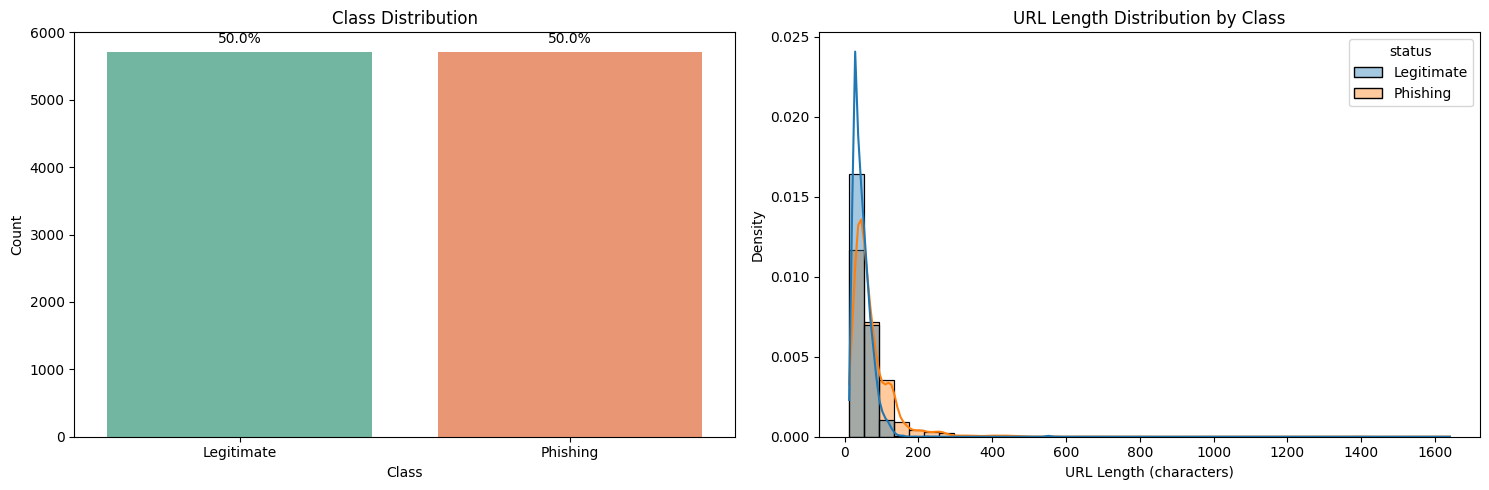
\includegraphics[width=0.95\textwidth]{model_visualizations/url_1.png}
\caption{URL dataset profile: class balance and URL-length distribution by class}
\end{figure}
\noindent\textit{This EDA view shows class balance and URL-length differences that make character-level features useful.}

\begin{figure}[H]
\centering
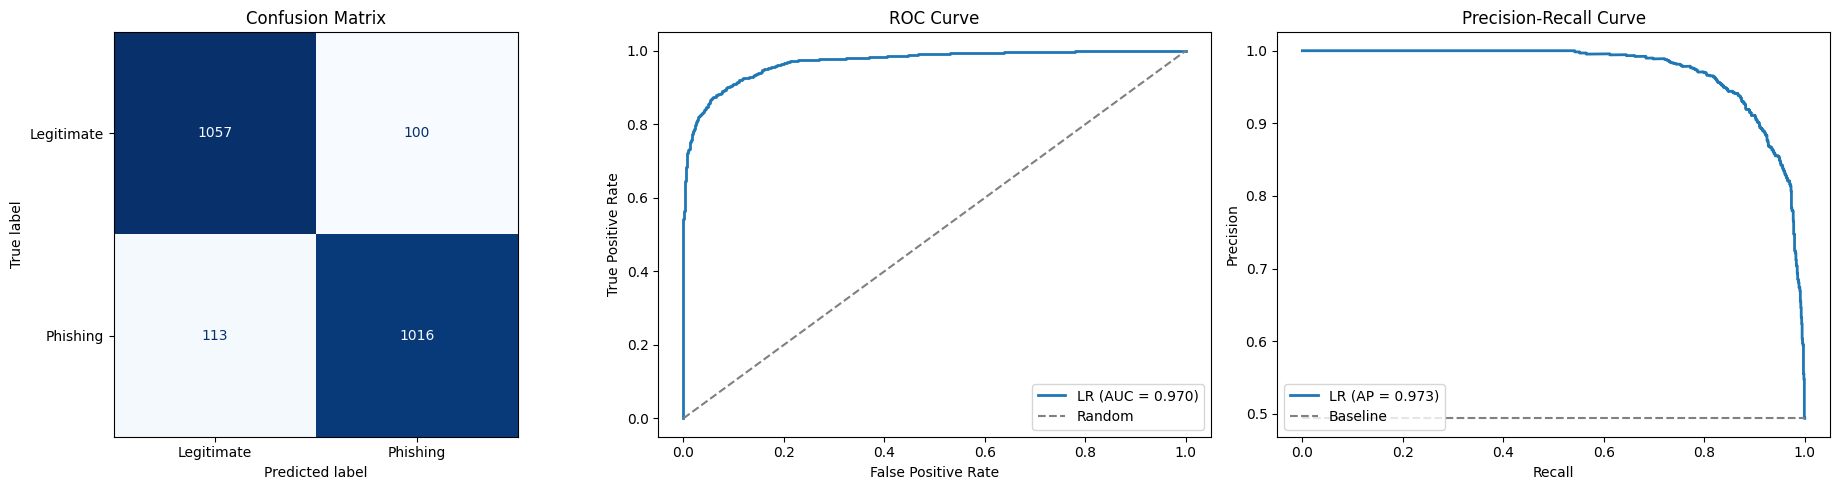
\includegraphics[width=0.95\textwidth]{model_visualizations/url_2.png}
\caption{Logistic Regression evaluation on hold-out split: confusion matrix, ROC, and precision-recall curves}
\end{figure}
\noindent\textit{Predicted labels and probabilities are used here to check class separation quality and phishing detection behavior.}

\begin{figure}[H]
\centering
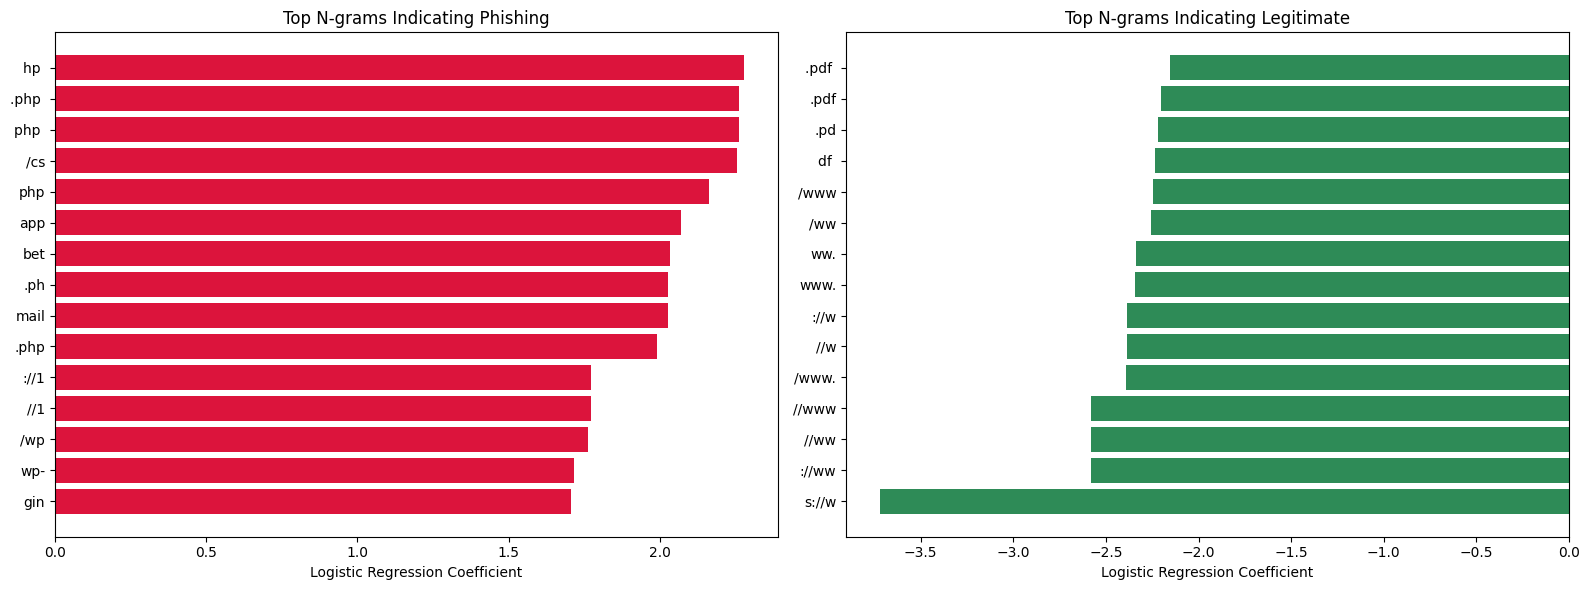
\includegraphics[width=0.95\textwidth]{model_visualizations/url_3.png}
\caption{Top character n-grams influencing the URL classifier}
\end{figure}
\noindent\textit{Positive coefficients point to phishing-leaning fragments, while negative coefficients align with legitimate URL patterns.}

\begin{figure}[H]
\centering
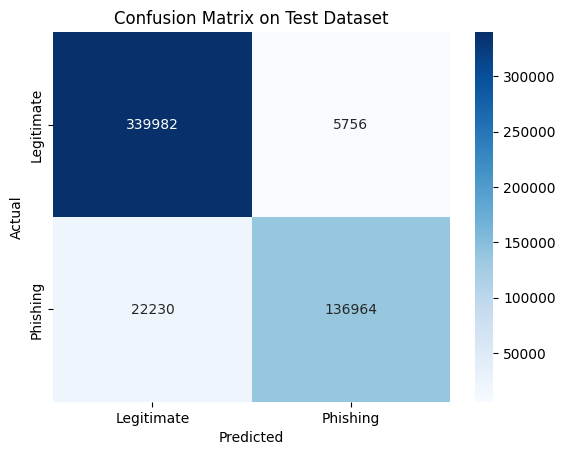
\includegraphics[width=0.55\textwidth]{model_visualizations/url_4.png}
\caption{External URL test-set confusion matrix}
\end{figure}
\noindent\textit{This confusion matrix comes from the separate test block using the same fitted vectorizer and trained classifier.}

\subsubsection{Email Pipeline Visualizations (\texttt{phishing\_email\_analysis\_bert.ipynb})}

\begin{figure}[H]
\centering
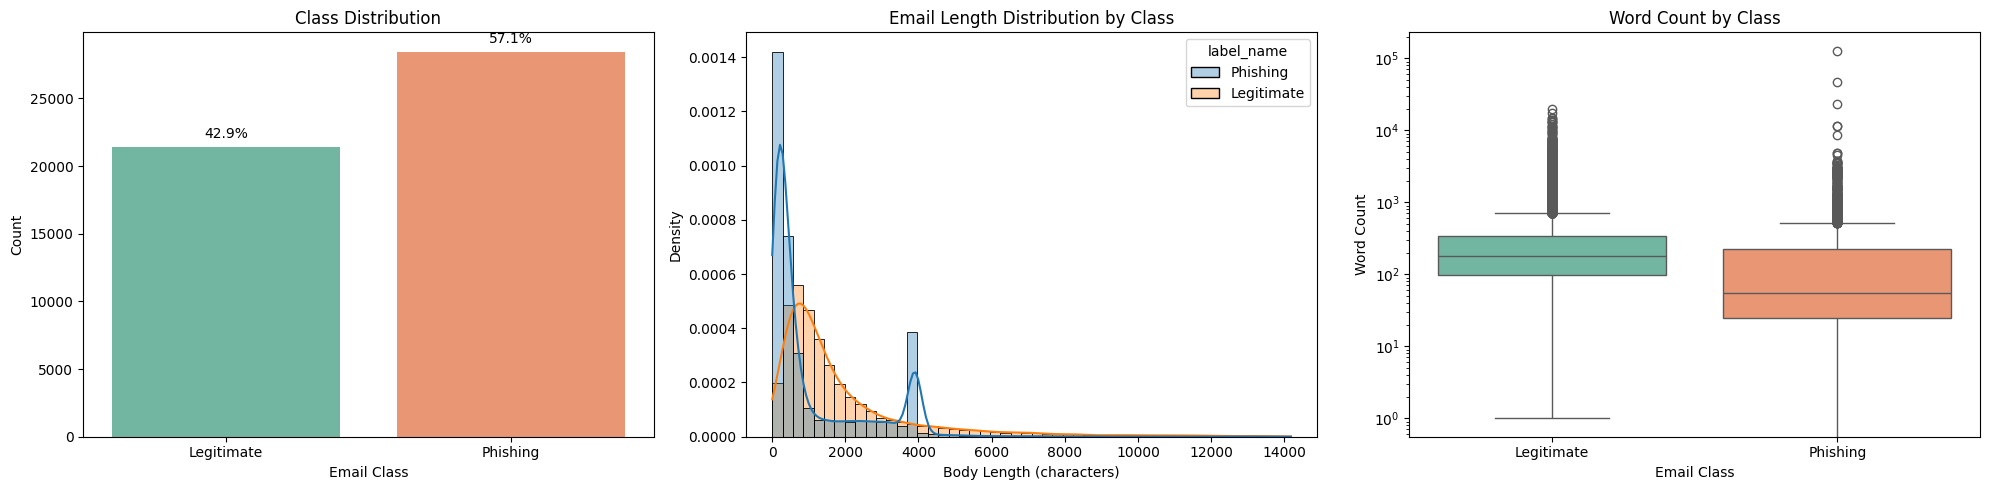
\includegraphics[width=0.95\textwidth]{model_visualizations/email_1.png}
\caption{Email dataset profile: class distribution, email-length distribution, and word-count spread}
\end{figure}
\noindent\textit{The dataset profile summarizes class ratio and message-length differences between legitimate and phishing emails.}

\begin{figure}[H]
\centering
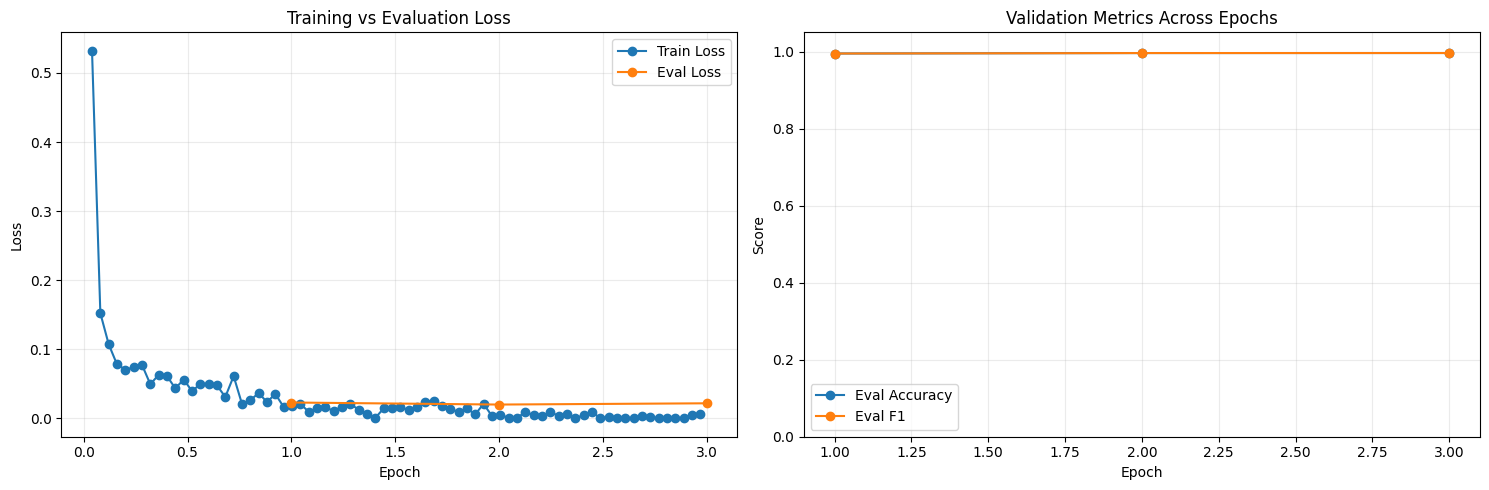
\includegraphics[width=0.95\textwidth]{model_visualizations/email_2.png}
\caption{DistilBERT training dynamics: train/eval loss and validation metrics across epochs}
\end{figure}
\noindent\textit{Built from trainer logs, these curves show convergence and the stability of validation accuracy and F1 across epochs.}

\begin{figure}[H]
\centering
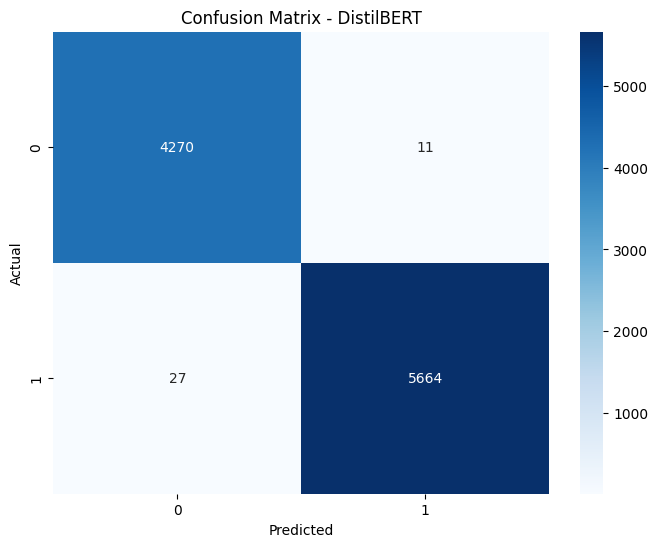
\includegraphics[width=0.55\textwidth]{model_visualizations/email_3.png}
\caption{DistilBERT confusion matrix on the combined hold-out split}
\end{figure}
\noindent\textit{The confusion matrix shows near-perfect class separation on the primary in-distribution split.}

\begin{figure}[H]
\centering
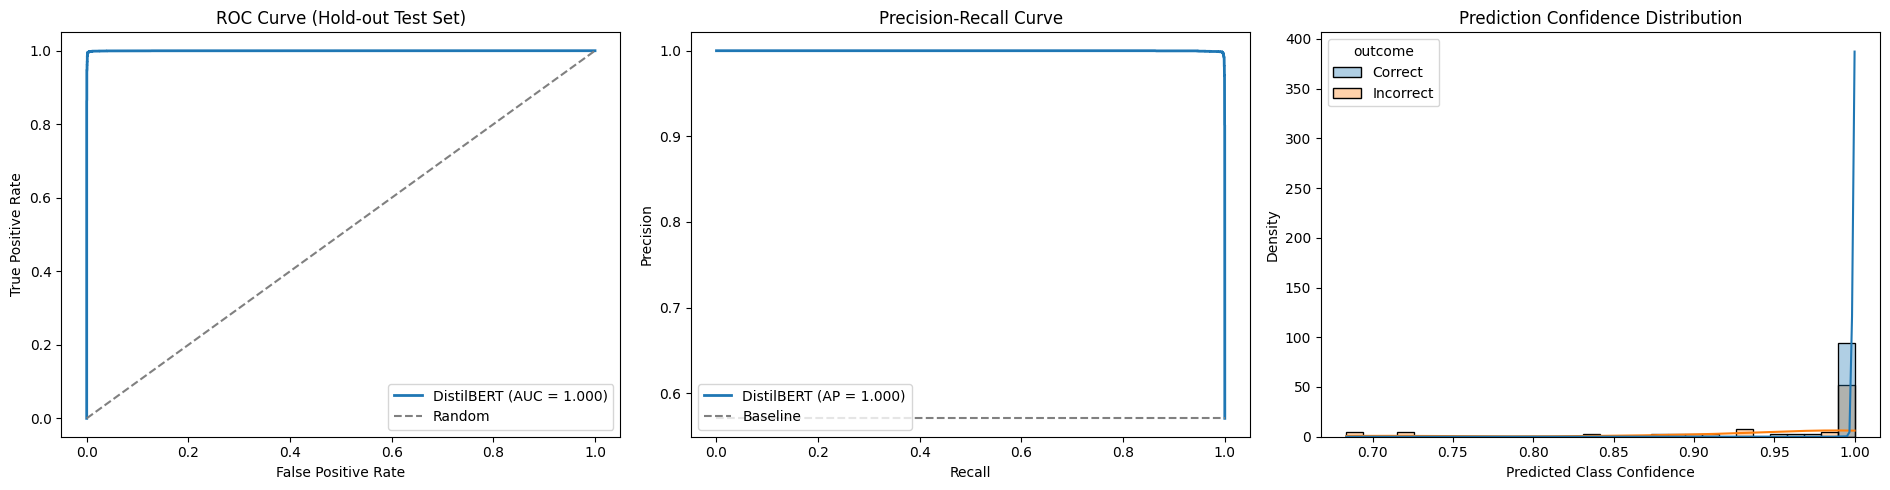
\includegraphics[width=0.95\textwidth]{model_visualizations/email_4.png}
\caption{DistilBERT probability diagnostics: ROC, precision-recall, and prediction-confidence distribution}
\end{figure}
\noindent\textit{Softmax probabilities from logits are used to inspect ranking quality and confidence behavior for correct and incorrect predictions.}

\begin{figure}[H]
\centering
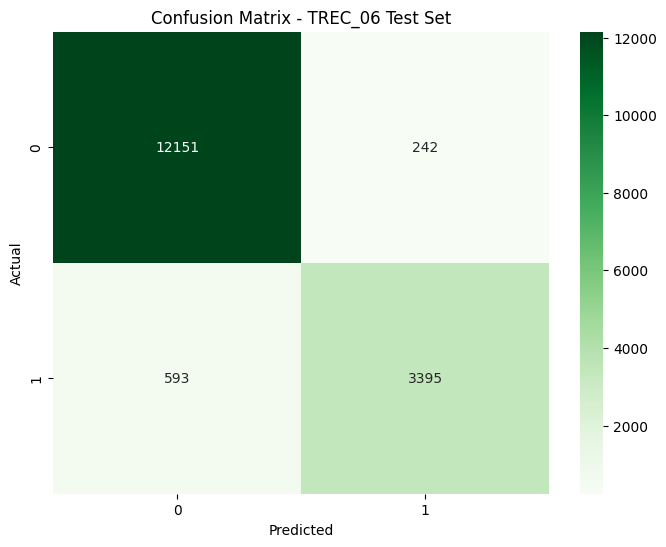
\includegraphics[width=0.55\textwidth]{model_visualizations/email_5.png}
\caption{DistilBERT confusion matrix on external TREC\_06 evaluation}
\end{figure}
\noindent\textit{This result comes from the dedicated TREC\_06 block and is used to check cross-source generalization.}

\section{System Output and Interface}
PhishTank is exposed through:
\begin{itemize}
    \item Browser extension with real-time URL checks and warnings
    \item API endpoints for URL and email prediction requests
\end{itemize}

\subsection{Threat Dashboard and URL Workflow}

\begin{figure}[H]
\centering
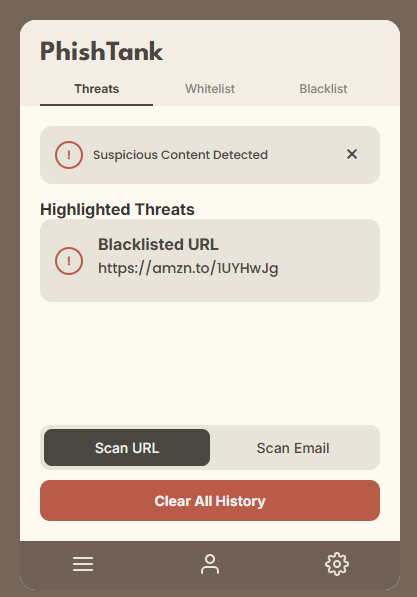
\includegraphics[width=0.32\textwidth]{screenshots/ui_1.png}
\caption{Threats tab with suspicious content alert and blacklisted URL highlight}
\end{figure}
\noindent\textit{The dashboard surfaces active warnings and shows detected malicious URLs in the highlighted threats panel.}

\begin{figure}[H]
\centering
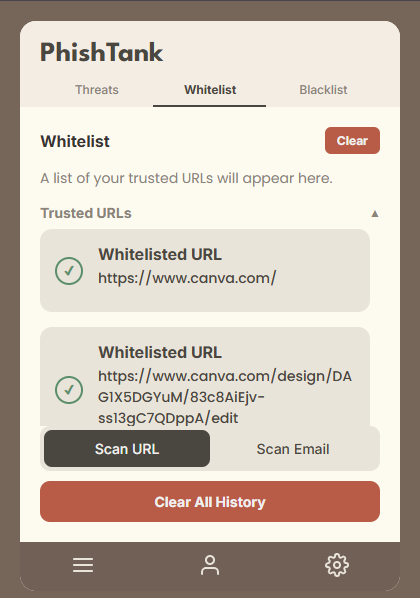
\includegraphics[width=0.32\textwidth]{screenshots/ui_2.png}
\caption{Blacklist tab showing blocked URL history}
\end{figure}
\noindent\textit{Users can review blocked URLs and remove entries from the blacklist view.}

\subsection{Email Scan Outcomes}

\begin{figure}[H]
\centering
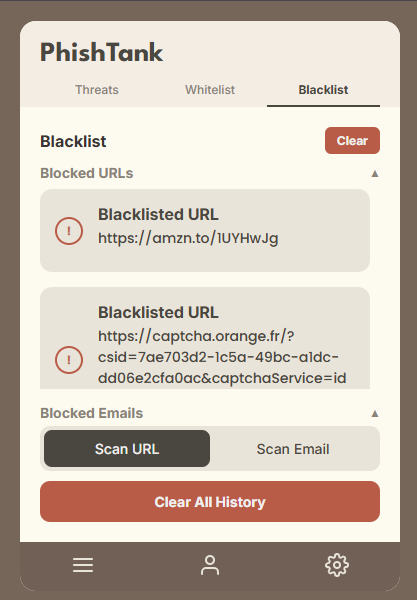
\includegraphics[width=0.32\textwidth]{screenshots/ui_3.png}
\caption{Email scan flow with legitimate classification toast}
\end{figure}
\noindent\textit{When DistilBERT predicts a safe email, the extension shows a confirmation toast and does not add the item to blacklist storage.}

\begin{figure}[H]
\centering
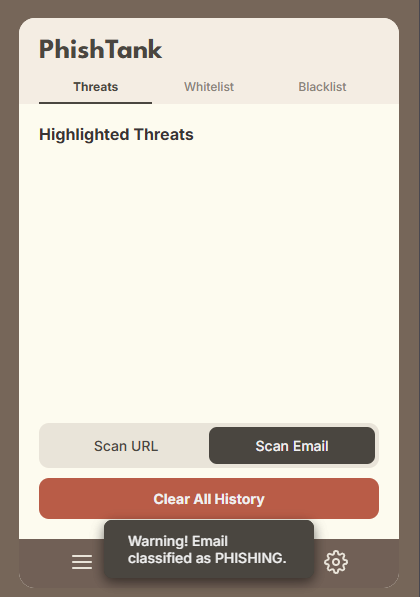
\includegraphics[width=0.32\textwidth]{screenshots/ui_5.png}
\caption{Email scan flow with phishing classification toast}
\end{figure}
\noindent\textit{A phishing prediction triggers a warning toast and marks the item for threat tracking.}

\begin{figure}[H]
\centering
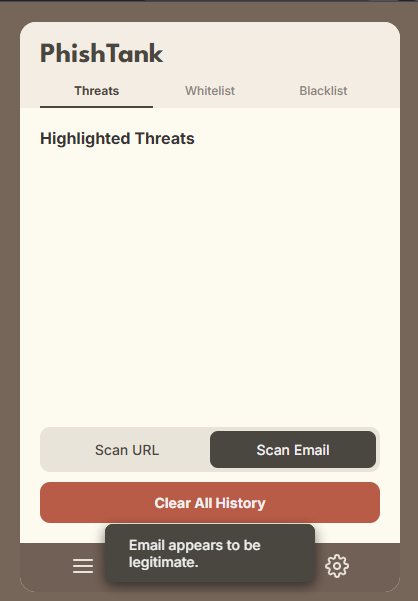
\includegraphics[width=0.32\textwidth]{screenshots/ui_4.png}
\caption{Blacklist email record with sender and suspicious content preview}
\end{figure}
\noindent\textit{Flagged emails are stored with sender metadata and a message preview so users can review them later.}

\subsection{Whitelist Management}

\begin{figure}[H]
\centering
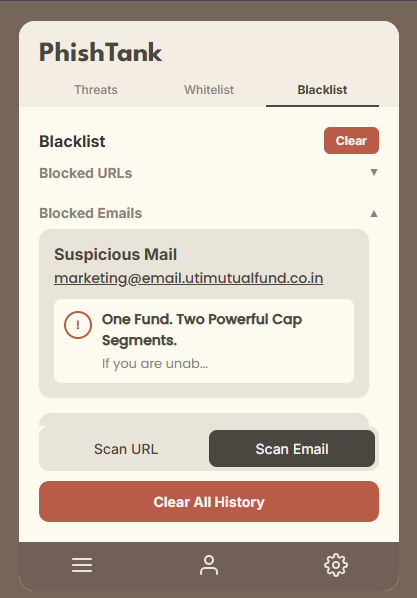
\includegraphics[width=0.32\textwidth]{screenshots/ui_6.png}
\caption{Whitelist tab showing trusted URL entries}
\end{figure}
\noindent\textit{Trusted URLs are listed separately so users can manage approved domains without turning off phishing checks.}

\section{Discussion}
The notebook results show that both pipelines perform well, especially the DistilBERT email model. For deployment, we still need to monitor:
\begin{itemize}
    \item Distribution shift in phishing strategies
    \item False positives on rare legitimate patterns
    \item Performance drift over time
\end{itemize}

Even with strong metrics in this project, periodic retraining and external validation are still necessary.

\section{Conclusion}
PhishTank demonstrates a practical phishing defense workflow that combines classical and deep learning models. The URL notebook provides a strong lightweight baseline, and the email notebook delivers very high classification performance on the curated split. With browser extension and API integration, the project works as an end-to-end phishing detection system.

\section{Future Work}
\begin{itemize}
    \item Automate periodic retraining with newly reported phishing samples
    \item Add calibration curves and threshold tuning for risk-sensitive deployment
    \item Expand multilingual email phishing detection
    \item Introduce explainability for both URL and email predictions
    \item Integrate blacklist and user-feedback loops into model updates
\end{itemize}

\section{References}
\begin{itemize}
    \item Project repository: \url{https://github.com/thirumuruganra/phishing-detection-system}
    \item Hugging Face Transformers documentation: \url{https://huggingface.co/docs/transformers}
    \item Scikit-learn documentation: \url{https://scikit-learn.org/stable/}
    \item FastAPI documentation: \url{https://fastapi.tiangolo.com/}
    \item DistilBERT model card: \url{https://huggingface.co/distilbert-base-uncased}
\end{itemize}

\end{document}
